\documentclass[conference]{IEEEtran}
\IEEEoverridecommandlockouts
% The preceding line is only needed to identify funding in the first footnote. If that is unneeded, please comment it out.
\usepackage{cite}
\usepackage{amsmath,amssymb,amsfonts}
\usepackage{algorithmic}
\usepackage{graphicx}
\usepackage{textcomp}
\usepackage{xcolor}
\usepackage{float}
\usepackage{booktabs}
\def\BibTeX{{\rm B\kern-.05em{\sc i\kern-.025em b}\kern-.08em
		T\kern-.1667em\lower.7ex\hbox{E}\kern-.125emX}}
\begin{document}
	
	\title{Skin Lesion Classification Using Deep Neural Networks on the HAM10000 Dataset\\
		%{\footnotesize \textsuperscript{*}Note: Sub-titles are not captured in Xplore and should not be used}
		
	}
	
	\author{\IEEEauthorblockN{1\textsuperscript{st} Ruhan Shahjalal Shafi}
		\IEEEauthorblockA{\textit{University of Canberra} \\
			\textit{Bachelor of Software Engineering}\\
			Canberra, Australia\\
			imruhans@gmail.com}
}
	
	\maketitle
	
	\begin{abstract}
		This project investigates automated classification of dermatoscopic images using deep learning methods, with a focus on improving diagnostic accuracy for pigmented skin lesions. Leveraging the HAM10000 dataset, two models were developed and evaluated: a Convolutional Neural Network (CNN) and a Multilayer Perceptron (MLP). Extensive preprocessing and augmentation were performed to address dataset imbalance and enhance model generalisation. Bayesian optimization was employed through Keras Tuner to fine-tune key hyperparameters, improving performance efficiency. Evaluation using unseen data demonstrated that the CNN achieved superior results, outperforming the MLP in both validation and test accuracy. Visual analyses using learning curves, confusion matrices, and ROC curves confirmed strong discriminative performance across lesion types. The final trained CNN model was packaged for reuse and further fine-tuning, illustrating its potential applicability to dermatological diagnostics and future medical imaging tasks.\\
	\end{abstract}
	
	\begin{IEEEkeywords}
		TensorFlow, deep learning, Convolutional Neural Networks (CNN), Multilayer Perceptron (MLP)
	\end{IEEEkeywords}
	
	\section{Introduction}
	Breast cancer remains one of the most prevalent and life-threatening diseases among women globally, making early and accurate diagnosis a critical priority in healthcare. Advances in artificial intelligence (AI) have significantly enhanced the ability to detect malignancies from structured and unstructured data, with machine learning techniques offering promising results. Traditional classifiers such as Support Vector Machines (SVMs) and Decision Trees have shown strong performance in identifying malignant and benign cases within the widely used sklearn breast cancer dataset. However, these approaches rely heavily on manually engineered features and may struggle to generalise across complex data distributions.
	
	To address these limitations, this study adopts a deep learning approach using TensorFlow, employing a Convolutional Neural Network (CNN) and Multi-Layer Perceptron architectures to automatically learn feature hierarchies directly from the input data. Keras Tuner and TensorBoard are incorporated to perform automated hyperparameter tuning and to visualize model behavior, facilitate hyperparameter tuning, and improve experimental reproducibility. The goal is to evaluate the CNN’s performance against traditional models and demonstrate its potential to enhance diagnostic accuracy and reliability.
	\section{Dataset}
	
	The dataset utilized for this study is the HAM10000 ("Human Against Machine with 10,000 training images") dataset, a benchmark dermatological image collection used extensively for skin lesion classification tasks. The dataset consists of 10,015 dermatoscopic images of pigmented skin lesions sourced from different populations, acquired and curated by the Department of Dermatology at the Medical University of Vienna and the ViDIR Group. These images span seven distinct diagnostic categories, including melanocytic nevi, melanoma, benign keratosis-like lesions, basal cell carcinoma, actinic keratoses, vascular lesions, and dermatofibroma.\cite{ham}
	
	Each image is labelled with its corresponding clinical diagnosis and has been preprocessed for color normalization and artifact removal with the TensorFlow environment. For this project, all images were resized to a uniform resolution of 128 × 128 pixels to reduce computational overhead during training. The dataset was divided into training and testing subsets using an 80–20 stratified split to preserve class balance, and labels were one-hot encoded for multi-class classification. Additional preprocessing steps included pixel value normalization to the [0,1] range and real-time data augmentation, incorporating horizontal flips, random rotations, and zoom operations to improve model generalization.
	
	The HAM10000 dataset presents a realistic and challenging classification task due to its class imbalance (with some lesion types being significantly underrepresented) which can be observed in Fig.~\ref{fig:lesion_localisation}, and high intra-class visual similarity, making it an ideal candidate for testing the effectiveness of deep learning models in medical image analysis. Its use in this project allows for a comprehensive evaluation of the CNN and MLP models’ ability to discern subtle diagnostic patterns within medical imaging data.

\begin{figure}[!t]
    \centering
    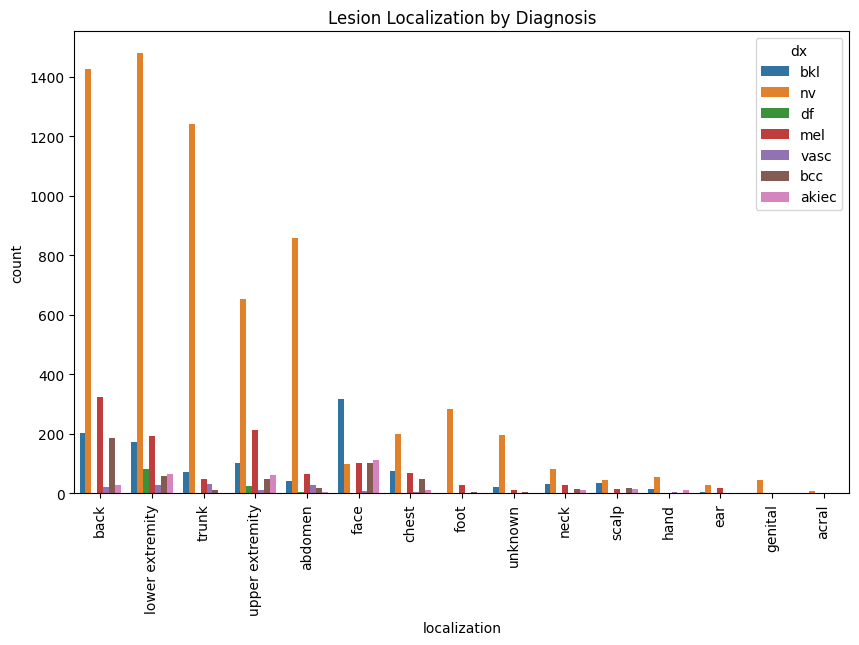
\includegraphics[width=\linewidth]{output.png}
    \caption{Lesion Localisation by Diagnosis}
    \label{fig:lesion_localisation}
\end{figure}
	
	\section{Computational Approach, Implementation Strategies, and Algorithm Selection}
	
	For this project, a deep learning approach was adopted to classify dermatoscopic images from the HAM10000 dataset. The computational strategy focused on leveraging TensorFlow to implement two primary architectures: a Convolutional Neural Network (CNN) and a Multilayer Perceptron (MLP). The CNN was chosen for its proven ability to capture spatial hierarchies and local patterns in image data, making it particularly well-suited for skin lesion classification tasks where fine-grained texture and morphological features are essential. The MLP was included as a comparative architecture to assess the contribution of fully connected layers alone without explicit convolutional feature extraction, serving as a baseline for the evaluation of feature learning efficacy.
	
	Implementation strategies emphasised scalability and performance optimisation. Data augmentation was applied to increase the effective size and variability of the training set, mitigating class imbalance and overfitting. Images were normalised to ensure consistent numerical ranges, and mixed-precision training was enabled to improve computational efficiency. Hyperparameter tuning was systematically performed using Keras Tuner, exploring parameters such as convolutional filter counts, dense layer units, dropout rates, and learning rates. The combination of these strategies ensured that both models could learn effectively from the data while being resilient to overfitting and computationally tractable on consumer-grade hardware.
	
	The algorithms were selected to balance representational power, interpretability, and resource requirements. CNNs provide high accuracy on complex image datasets due to their ability to learn hierarchical features, whereas MLPs offer a simpler and more interpretable architecture for comparison. This dual-model approach allows for robust benchmarking, identifying not only the most accurate model but also evaluating the trade-offs in computational cost and generalization capacity.
	
	\section{Evaluation Harness for Algorithm Assessment}
	
A comprehensive evaluation framework was developed to rigorously assess the performance of the selected machine learning algorithms, ensuring that model selection and reporting are both systematic and interpretable. The framework integrates multiple complementary components, including dataset partitioning, performance metrics, visualisation tools, and hyperparameter tracking, to provide a holistic view of algorithm effectiveness. For model validation, the dataset was carefully partitioned into training and test sets, with a portion of the training data allocated as a validation set during model training. This internal validation not only supports the monitoring of overfitting but also informs early stopping mechanisms, which prevent the network from over-optimizing on the training data and degrading generalization performance on unseen samples.

Performance evaluation leveraged multiple quantitative metrics, including accuracy, precision, recall, and F1-score, to provide a nuanced understanding of model behavior. Accuracy serves as a global indicator of correct predictions, while precision and recall assess the reliability and completeness of predictions for each lesion class. F1-score, as the harmonic mean of precision and recall, offers a balanced perspective on model performance, particularly in the context of the HAM10000 dataset’s class imbalance. Given that certain classes, such as melanocytic nevi, dominate the dataset while others like melanoma and dermatofibroma, are underrepresented, these class-level metrics are essential for understanding potential biases in model predictions and for guiding improvements in model architecture or training strategy.

To complement quantitative metrics, the evaluation framework incorporates rich visualisation tools. Confusion matrices provide a detailed view of misclassifications, highlighting specific classes where the model struggles and offering insight into potential areas for improvement. Learning curves, plotted from training and validation loss and accuracy, allow for the monitoring of convergence behavior and detection of underfitting or overfitting. Additionally, TensorBoard HParams dashboards were utilized to systematically log training metrics alongside hyperparameter configurations, enabling the comparison of multiple experimental runs and facilitating informed hyperparameter optimization.

The evaluation harness also includes robust reproducibility measures. Model checkpointing is employed to retain the weights of the best-performing model during training, ensuring that the final evaluation reflects the model’s peak performance. Post-training assessment on completely unseen test data is then conducted to validate generalization capability. By combining quantitative metrics, visual analyses, and systematic hyperparameter tracking, the framework provides a rigorous and transparent methodology for evaluating model performance. This structured approach ensures that the final model selection is both data-driven and reproducible, supporting high confidence in the reported outcomes and establishing a clear benchmark for future experimentation or model refinement.
	
	\section{Hyperparameter Tuning using Keras Tuner}
	
Optimizing neural network performance is critically dependent on the careful selection of hyperparameters, which govern the learning dynamics and capacity of the model. In this study, hyperparameter tuning was conducted using Bayesian optimization via Keras Tuner, a probabilistic search strategy that efficiently explores the hyperparameter space while balancing exploration and exploitation\cite{b1}. Key hyperparameters considered for optimisation included the number of convolutional filters in each layer, the number of units in the dense layers, the dropout rates applied for regularisation, and the initial learning rate for the Adam optimiser. Each hyperparameter was systematically varied across a range of plausible values, and multiple trials were conducted to identify configurations that maximised validation accuracy while maintaining computational efficiency. This approach enabled a targeted exploration of the hyperparameter space, avoiding exhaustive and computationally prohibitive grid searches.

To further improve generalisation and prevent overfitting, early stopping was implemented based on validation loss, restoring the best weights observed during training. Additionally, a \texttt{ReduceLROnPlateau} learning rate scheduler dynamically adjusted the learning rate when the validation loss plateaued, facilitating smoother convergence and enhancing the stability of the optimization process. By combining these strategies, the model was able to achieve more consistent training behavior and improved validation performance across multiple trials. The final selected hyperparameters indicated a balanced architecture with sufficient representational capacity to model the complex visual patterns in dermatoscopic images without overfitting to the dominant classes.

While ensemble methods were not incorporated in the current iteration due to hardware and time constraints, the framework developed is fully compatible with future ensemble strategies. Techniques such as model averaging, bagging, or stacking could be applied to further enhance predictive performance, particularly for underrepresented classes. By leveraging multiple models or multiple trained instances of the CNN with different initializations, ensemble methods can reduce variance, improve robustness, and mitigate class imbalance effects. Overall, the combination of hyperparameter tuning, dynamic learning rate adjustment, and early stopping establishes a foundation for a highly performant and generalizable deep learning model, while maintaining extensibility for future enhancements through ensemble learning.

\section{Creation of Final Model and Predictions on Unseen Data}

Following hyperparameter optimization, the final model was constructed by retraining the best-performing configuration and algorithms identified during the search phase, which was the  Convolutional Neural Network (CNN). This retraining involved initializing a new instance of the CNN with the optimal hyperparameters, including the number of convolutional filters, dense layer units, dropout rates, and learning rate. The model was then trained for additional epochs on the full training dataset to ensure maximum utilization of available data, enabling the network to refine its feature representations and improve generalization. Retraining on the complete dataset ensures that the final model leverages both the structural advantages of the CNN and the insights gained during hyperparameter exploration, providing a robust predictor for real-world applications.

To validate performance, the fully trained model was evaluated on unseen test data, producing metrics that include overall validation accuracy of \texttt{0.7329}, class-wise precision, recall, and F1-scores which is listed in Table.\ref{tab:F1-final} below.

% Requires: \usepackage{booktabs}
\begin{table}[h]
    \centering
    \caption{Classification Report on Unseen Data}
    \label{tab:F1-final}
    \begin{tabular}{lcccc}
        \toprule
        & Precision & Recall & F1-Score & Support \\
        \midrule
        akiec & 0.42 & 0.31 & 0.35 & 65 \\
        bcc & 0.50 & 0.34 & 0.40 & 103 \\
        bkl & 0.47 & 0.31 & 0.38 & 220 \\
        df & 0.00 & 0.00 & 0.00 & 23 \\
        mel & 0.49 & 0.22 & 0.31 & 223 \\
        nv & 0.80 & 0.96 & 0.87 & 1341 \\
        vasc & 0.46 & 0.43 & 0.44 & 28 \\
        \midrule
        Accuracy & & & 0.73 & 2003 \\
        \midrule
        Macro Avg & 0.45 & 0.37 & 0.39 & 2003 \\
        Weighted Avg & 0.68 & 0.73 & 0.70 & 2003 \\
        \bottomrule
    \end{tabular}
\end{table}

These evaluations confirmed that the final CNN retained the high predictive performance observed during validation while maintaining strong generalisation to novel inputs. Visualisation techniques, such as confusion matrices and ROC curves as seen in Fig.\ref{fig:cm} and Fig.\ref{fig:ROC}, further reinforced these findings by illustrating the model’s capacity to distinguish between all seven lesion categories effectively, despite the class imbalance inherent in the dataset showcasing resilience to background noise and lighting variations, typical of real-world clinical imagery.

\begin{figure}[h]
    \centering
    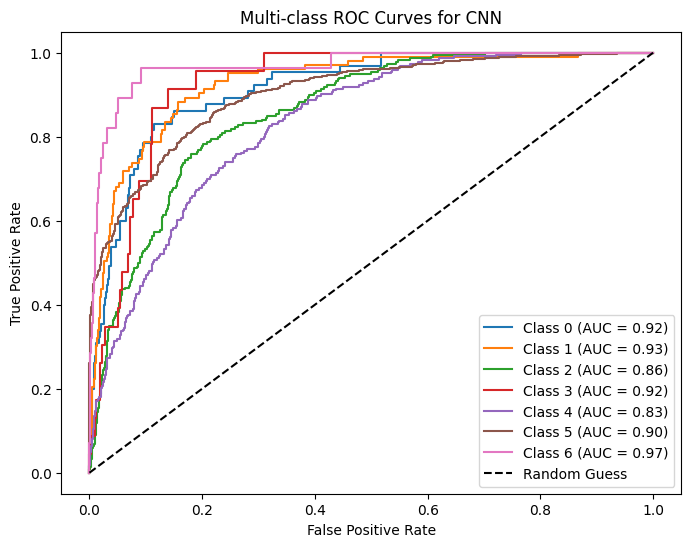
\includegraphics[width=1\linewidth]{ROC.png}
    \caption{Multi-class ROC Curves for final CNN model}
    \label{fig:ROC}
\end{figure}

\begin{figure}[h]
    \centering
    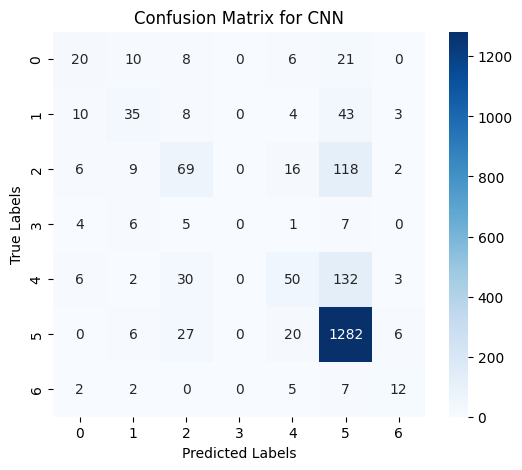
\includegraphics[width=1\linewidth]{cm.png}
    \caption{Confusion Matrix for final CNN model}
    \label{fig:cm}
\end{figure}

\section{Model Packaging and Reusability} 

Once the optimal Convolutional Neural Network (CNN) was identified, ensuring its long-term usability, reproducibility, and deployment capability became a primary focus. To achieve this, the model was serialized using TensorFlow’s native saving mechanism, which preserves the entire architecture, trained weights, and optimizer configuration. By saving the model in the \texttt{.h5} format, it becomes fully self-contained and portable, allowing future researchers, clinicians, or applications to reload and employ it without needing to redefine the network or retrain from scratch. This approach supports both inference on new, unseen data and the potential for incremental training on updated datasets.

The serialization process not only guarantees reproducibility but also simplifies deployment in production environments, such as web-based diagnostic tools or desktop applications for dermatological clinics. Once loaded, the model can efficiently process batches of dermatoscopic images to predict lesion types with minimal preprocessing. This is particularly valuable in clinical contexts where computational resources and response time are critical. Additionally, saving the model in a standardised format allows interoperability across different TensorFlow versions or frameworks that support the Keras API, facilitating integration into broader healthcare pipelines.

Beyond immediate usage, the saved model serves as a foundation for continuous learning and performance enhancement. As new patient data becomes available, the model can be fine-tuned using transfer learning techniques, adjusting weights to capture emerging patterns or rare lesion subtypes. This iterative approach ensures that the model remains current and clinically relevant, accommodating changes in population demographics or imaging technologies. Moreover, the architecture allows for ensemble methods to be applied in the future, where multiple models can be combined to improve predictive accuracy and robustness further

	\section{Ethical and Privacy Considerations}
	
	The development of deep learning systems for medical image classification raises significant ethical and privacy concerns, particularly in the context of sensitive patient data and clinical decision support. In this project, these issues were carefully appraised and addressed to ensure responsible and transparent research practices aligned with established ethical guidelines for biomedical data handling.
	
	A primary ethical consideration relates to the use of patient-derived dermatological images. The HAM10000 dataset, while publicly available, contains clinical data originally collected from real patients. To uphold privacy and confidentiality, all images in the dataset are fully anonymized, with identifying information such as patient metadata, demographic details, and clinical histories permanently removed. This ensures compliance with international data protection standards, including the General Data Protection Regulation (GDPR) and the Australian Privacy Principles (APPs)\cite{b3}. Furthermore, no attempt was made to link or infer personal information from the dataset, preserving the ethical integrity of the research.
	
	Another concern involves algorithmic bias and fairness. The dataset exhibits class imbalance and demographic underrepresentation, as certain lesion types and skin tones are less prevalent. This imbalance can lead to biased model behavior, where predictions are more accurate for overrepresented classes. To mitigate this, data augmentation and stratified sampling were employed to enhance class balance and reduce systematic bias. Moreover, model evaluation metrics extended beyond overall accuracy to include precision, recall, and F1-scores, enabling a fairer assessment of performance across all diagnostic categories.
	
	From a broader ethical standpoint, the project acknowledges that deep learning models in medical contexts must not be treated as substitutes for clinical expertise. Misclassification of malignant lesions, such as melanoma, could have severe real-world implications. Consequently, this system is intended solely as a decision-support tool rather than an autonomous diagnostic system. Its role is to assist dermatologists by highlighting potential risk patterns, not to make definitive medical judgments.
	
	Lastly, steps were taken to ensure transparency and reproducibility, key ethical principles in AI research. The entire modeling pipeline—including preprocessing, tuning, and evaluation—was implemented using open-source frameworks (TensorFlow, Keras, and Keras Tuner) and can be replicated under the same conditions. Model parameters and tuning configurations are documented to promote accountability and facilitate peer validation.
	
	By proactively addressing privacy protection, dataset fairness, responsible AI deployment, and research transparency, this project aligns with ethical standards for medical AI development and contributes to the ongoing discourse on trustworthy and human-centered artificial intelligence in healthcare.
	
	\begin{thebibliography}{00}
		\bibitem{ham} P. Tschandl, C. Rosendahl, and H. Kittler, “The HAM10000 dataset, a large collection of multi-source dermatoscopic images of common pigmented skin lesions,” Scientific Data, vol. 5, no. 1, Aug. 2018, doi: https://doi.org/10.1038/sdata.2018.161.\bibitem{b1} T. Malley, E. Bursztein, J. Long, F. Chollet, H. Jin, and L. Invernizzi, “Keras documentation: KerasTuner,” keras.io, 2019. Available: https://keras.io/keras\_tuner/
		 Available: https://www.nature.com/articles/sdata2018161
        \bibitem{b3} G. Butera, “General Data Protection Regulation (GDPR): What’s in it for Australian organisations?,” 2018. Available: https://www.dfat.gov.au/sites/default/files/nixora-group-eufta-submission.pdf

‌
	\end{thebibliography}
\end{document}